\begin{abstract}
Machine learning classifiers with high test accuracy often perform
poorly under adversarial attacks.
It is commonly believed that 
%, i.e. they have high \emph{robust} error.
adversarial training %is commonly believed to
alleviates this issue.
%effectively decrease the robust error. 
In this paper, we demonstrate that,
surprisingly, the opposite may be true --- Even though adversarial training helps when enough data is  available, it may hurt robust generalization in the small sample size regime. 
%We show that adversarial training
%with perceptible attacks can hurt robust generalization on 
We first prove this phenomenon for a high-dimensional linear
classification setting with noiseless observations. Our proof provides explanatory insights that may also transfer to feature learning models. 
%Specifically, when SGD on the robust logistic loss is run until convergence, 
%Specifically we show that the robust error of the robust max-margin solution monotonically increases with increasing training perturbation
%strength set size $\epsilon$, starting from standard training ($\epsilon =
%0$). 
%In particular, this drop is more pronounced for small sample sizes. 
Further, we observe in experiments on standard image datasets that the same behavior occurs %in the small sample size regime 
for perceptible attacks
that effectively reduce class information such as mask attacks and object corruptions. 
%This paper provides an example how common beliefs may need to be revisited
\end{abstract}

\section{Introduction}
\label{sec:intro}
\begin{wrapfigure}{r}{0.43\textwidth}
\centering
\vspace{-0.1in}
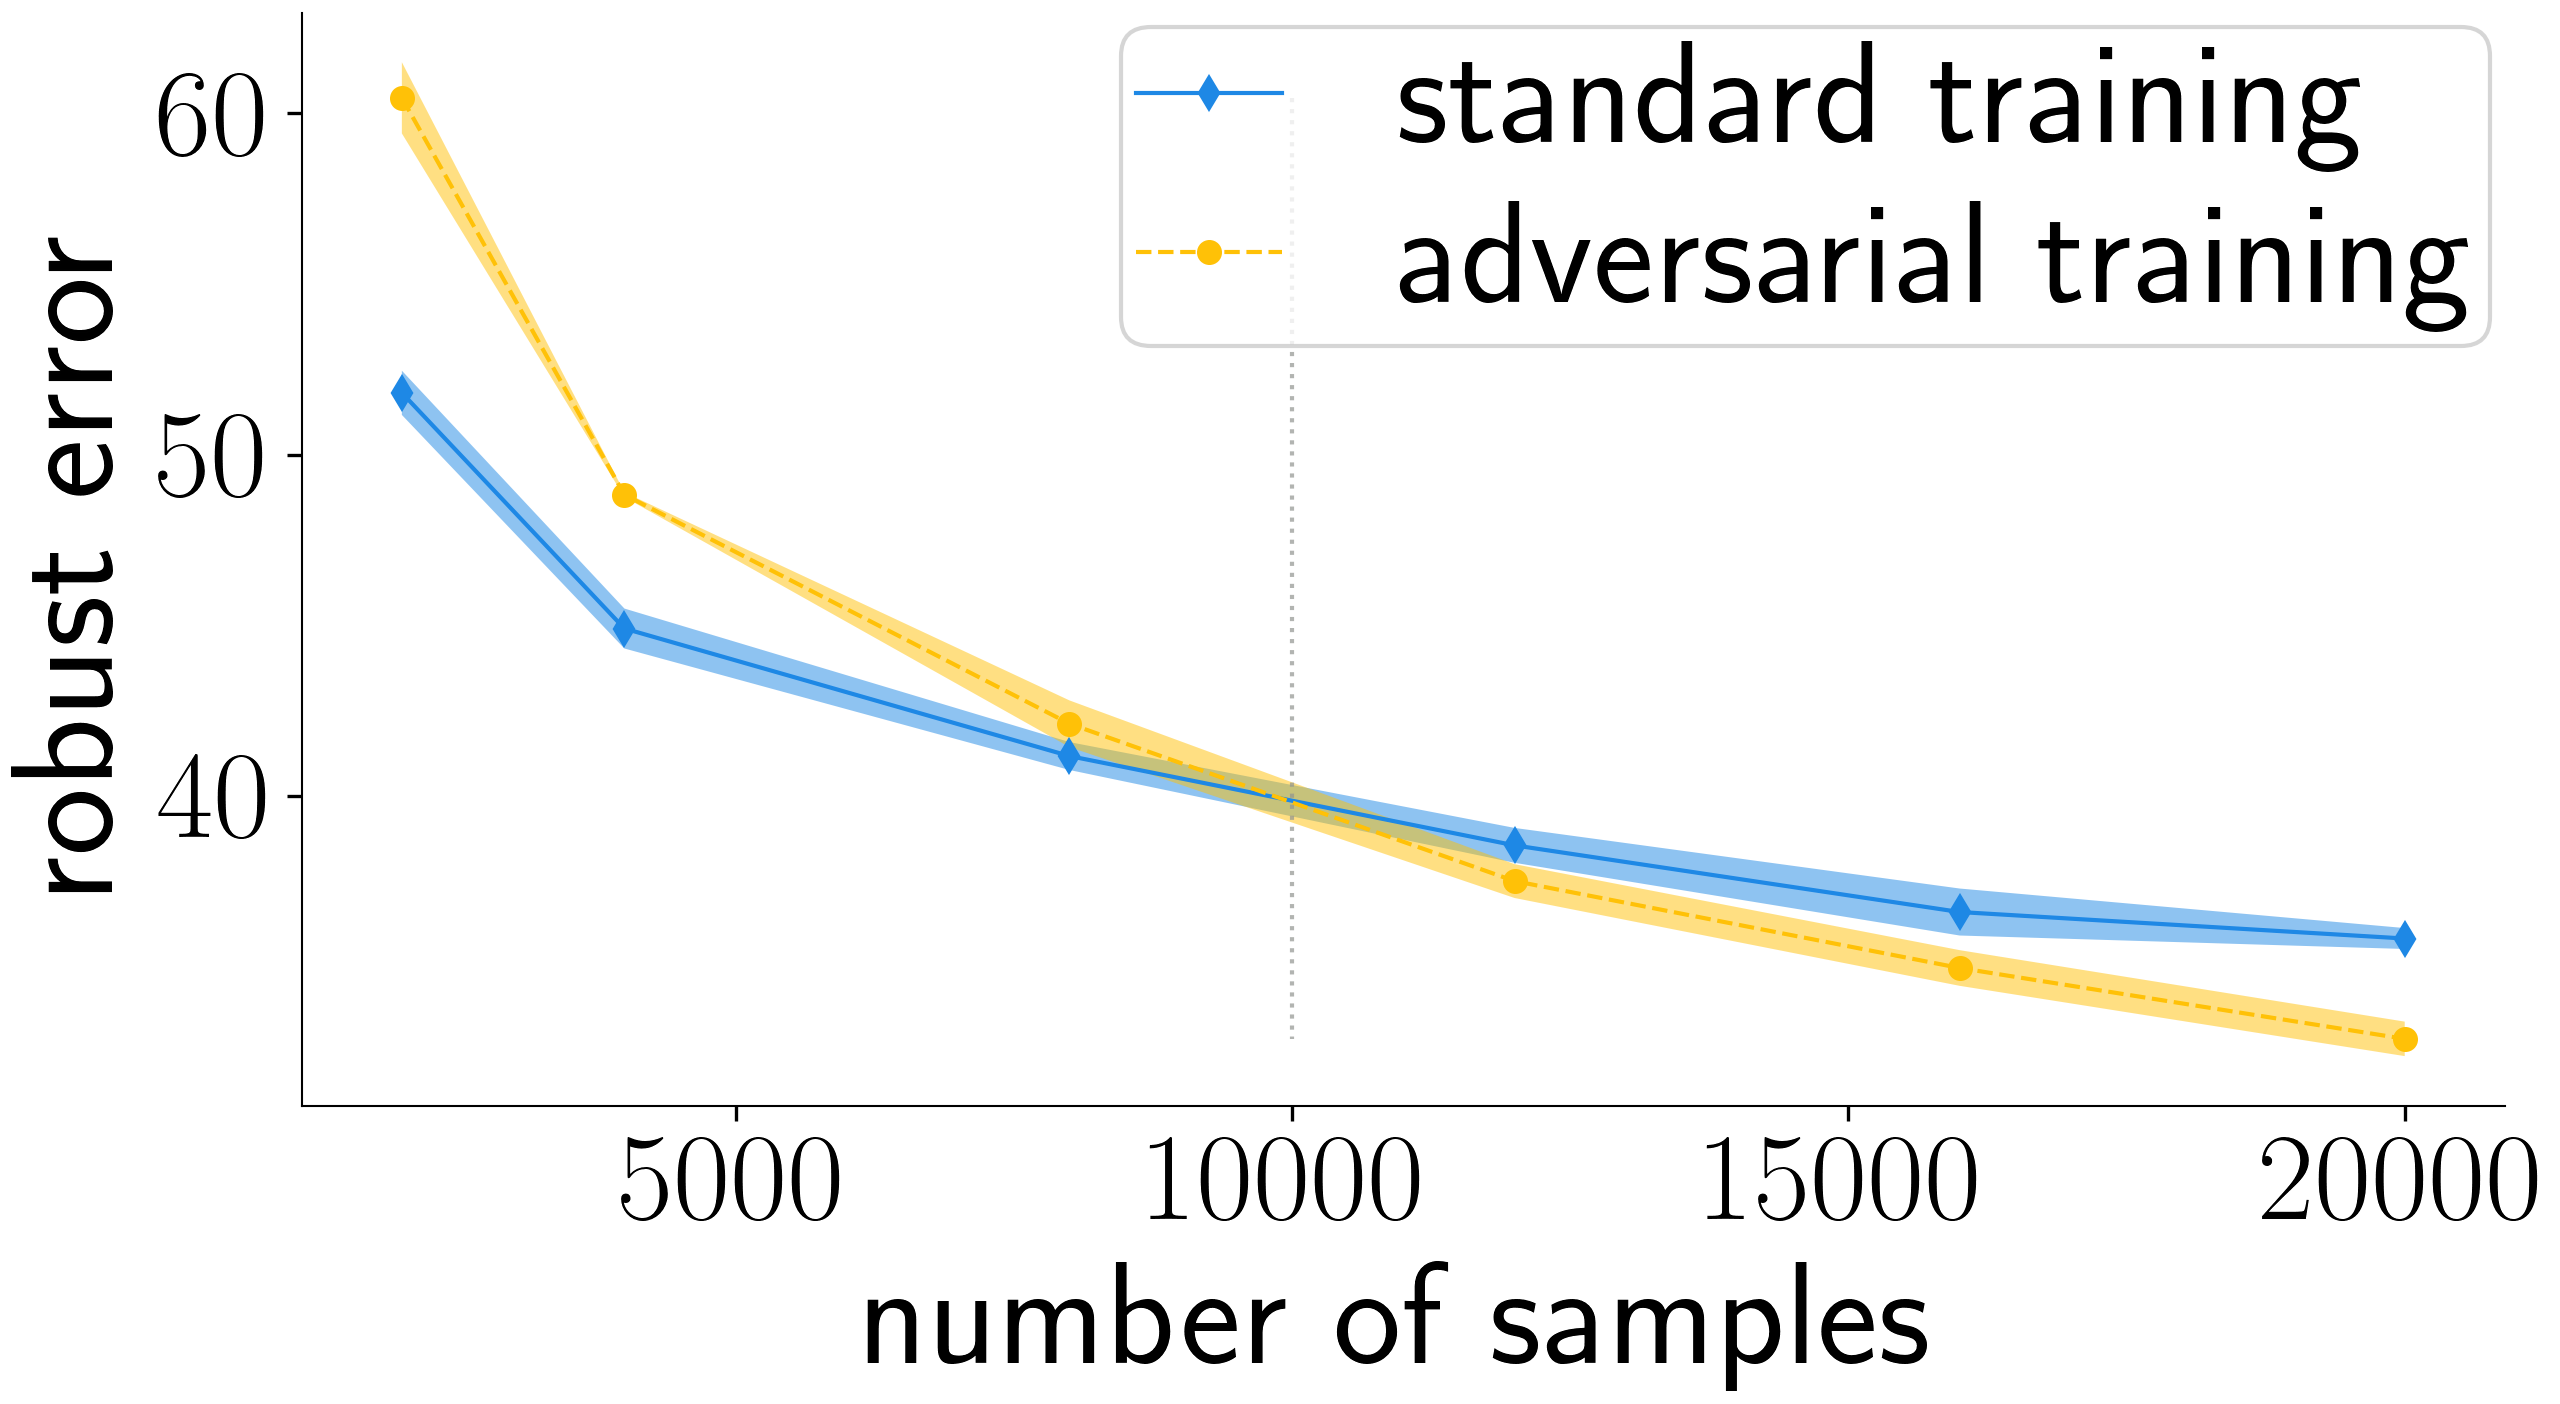
\includegraphics[width=0.99\linewidth]{plotsAistats/teaser_try_2.png}
\caption{
  %The robust error of standard and adversarial training as a function of sample size on subsampled datasets from \mbox{CIFAR10} attacked with $2\times2$ masks.
  On subsampled \mbox{CIFAR10} attacked by $2\times 2$ masks, adversarial training yields higher robust error than standard training
  when the sample size is small, even though it helps for large sample sizes.
  (see Sec.~\ref{sec:app_cifar10} for details).}
  %We subsample \mbox{CIFAR10} and perform $2\times 2$ mask attacks }
  %hurts robust generalization when the sample size is small, even though it helps for large sample sizes. For experimental details see Section~\ref{sec:app_cifar10}.}
  \vspace{-0.2in}
\label{fig:teaserplot}
\end{wrapfigure}

Today's best-performing classifiers are vulnerable to adversarial attacks
\cite{goodfellow15, szegedy14} and exhibit high \emph{robust error}: for many inputs, their predictions change under adversarial perturbations,
%for worst-case perturbed inputs
even though the true class stays the same. 
%For images for example,
For example, in image classification tasks, we distinguish between two categories of
such attacks that are content-preserving \cite{gilmer18b} (or consistent \cite{raghunathan20}) if their strength is limited --- perceptible and imperceptible perturbations.
Most work to date studies imperceptible attacks such as 
bounded $\ell_p$-norm perturbations \cite{goodfellow15, madry18, moosavi16}, small transformations using image processing
techniques \cite{ghiasi19, zhao20, laidlaw21, Luo18} or 
nearby samples on the data manifold \cite{Lin20, Zhou20}.
%with a perceptible distance measured using image processing metrics 
They can often use their limited budget to successfully fool a learned classifier but, by definition, do not visibly reduce information about the actual class: the object in the perturbed image looks exactly the same as in the original version.

On the other hand, perceptible perturbations may occur more naturally in practice or are physically realizable. 
For example, stickers can be placed on traffic signs \cite{Eykholt18},
%or street signs
%or 
masks of different sizes may cover important features of human faces
\cite{Wu20}, images might be rotated or translated \cite{Logan19},
%Furthermore, 
animals in motion may appear blurred in photographs
depending on the shutter speed, or the lighting conditions could be poor (see Figure~\ref{fig:sig_att_examples}).
Some perceptible attacks can effectively
use the perturbation budget to reduce actual class information
in the input (the \emph{signal}) while still preserving the original class.
For example, a stop sign with a small sticker doesn't lose its semantic meaning
or a flying bird does not become a different species because it induces motion blur
in the image.
We refer to these attacks as \emph{\nameofattacks} (see
Section~\ref{sec:robustness} for a more formal
characterization). 

In this paper, we
demonstrate that one of the most common beliefs 
for adversarial attacks does not transfer to \nameofattacks, in
particular when the sample size is small. Specifically, it is widely acknowledged that adversarial training often achieves significantly lower adversarial error than standard
training. This holds in particular if %it uses 
the perturbation type 
\cite{madry18, zhang19, Bai21} and perturbation budget match the attack during test time. 
Intuitively, the improvement is a result of decreased
\emph{attack-susceptibility}: independent of the true class,
adversarial training explicitly encourages the classifier to predict
the same class for all perturbed points.

%% a general widespread practice to defend against
%%  adversarial perturbation \fy{types} do not transfer to \nameofattacks, in
%% particular when the sample size is small.

%% that can more 
%% efficiently use the perturbation budget to reduce actual class information
%% in the input (or \emph{signal} in short) while preserving the actual class.

%% may be  imperceptible to the human eye
%% %(e.g. small $\ell_p$-norm perturbations),
%% or perceptible and physically realizable (e.g. rotations.


%% For example, stickers can be placed on traffic signs \cite{Eykholt18}
%% %or street signs
%% or masks of different sizes may cover important features of human faces
%% \cite{Wu20}. Images might be rotated or translated \fy{cite}.
%% Furthermore, animals in motion may appear blurred in photographs
%% depending on the shutter speed, or the lighting conditions could be poor (see Figure~\ref{fig:sig_att_examples}).
%% Usually, the distribution of such
%% transformations is not known or observed so that we cannot ``simply''
%% solve a domain adaptation problem \fy{sounds like distribution over all these types of perturbations}. - if you wanna cut this, can move to directed attacks section


%What all of the above examples have in common is that they


%% Most previous work in the literature to date studies imperceptible attacks \fy{such as blablabla $\ell_p$ balls, image processing techniques, manifold -- add}: 
%% they can often use their limited budget to successfully fool the classifier but, by definition, do not visibly reduce class information.
%% %% for example, 
%% %% $\ell_p$-perturbations can efficiently use a small budget to
%% %% fool a given classifier without visibly altering the image
%% %% for humans.
%% In contrast, we consider \emph{perceptible attacks} that can more 
%% efficiently use the perturbation budget to reduce actual class information
%% in the input (or \emph{signal} in short) while preserving the actual class.
%% For example, a stop sign with a small sticker doesn't lose its semantic meaning
%% or a bird does not become a different species when it flies and causes motion blur
%% in the image.
%% %directed attacks 
%% %most efficiently use the perturbation budget to reduce the information about the class in the input (referred to signal in short).
%% We refer to these attacks as \emph{\nameofattacks} (see
%% Section~\ref{sec:robustness} for a more formal
%% characterization). \fy{hm not REALLY true :/} In this paper, we
%% demonstrate that some widespread practices to defend against
%% other adversarial perturbation \fy{types} do not transfer to \nameofattacks, in
%% particular when the sample size is small.

%% $\ell_p$-perturbations, which are undirected:
%% they most efficiently use the budget to fool a particular classifier. This (in turn) can be quite inefficient to reduce the actual “signal”.
%% %In particular, $\ell_p$-ball perturbations are not \nameofattacks as they use all directions causing missclassification.
%% %% these are far from the only attacks that could happen
%% %% in practice \cite{gilmer18b}.
%% In this paper, we demonstrate that some widespread common practices for
%% $\ell_p$-ball perturbations do not transfer to \nameofattacks.


%% In this paper, we generally consider perceptible attacks that 
%% efficiently use the perturbation budget to reduce class information
%% in the input (or \emph{signal} in short). 
%% %directed attacks 
%% %most efficiently use the perturbation budget to reduce the information about the class in the input (referred to signal in short).
%% We refer to these attacks as \emph{\nameofattacks} and refer to Section~\ref{sec:robustness} for a more detailed discussion.


%specifically
%target the ground truth signal, referred to as \emph{\nameofattacks} (see Section~\ref{sec:robustness} for an extended discussion).

%% robustness more generally against attacks \fy{can't parse: that are constrained on the ground truth signal}, which we refer to as \emph{\nameofattacks} (more
%% detail in Section~\ref{sec:robustness}).

%% \fy{above is a more concise version of below}
%% \fy{more concise, criminal face detection could be made a running
%%   example if exps go through, currently the safety-critical aspect is
%%   slightly missing, we just say we wanna be able to detect no matter
%%   which transformation - do we want to make it safety-critical?}  For
%% example, animals could be moving at different speeds, causing motion
%% blur (which also depends on the camera settings that might differ
%% between photographers). Or a spreading respiratory disease might cause
%% important features of the face to be covered by a mask of certain
%% size.  For animals or face detection, an optimally robust model should
%% recognize the objects irrespective of such transformations
%% \fy{perturbations} since the objects identity is unchanged (in other
%% words consistent/content-preserving). If the distribution of such
%% changes were known or observed, one could optimize the loss on that
%% shifted distribution by using tools from domain adaptation \fy{cite}.
%% Usually however, the distribution is unknown in which case
%% distribution shift or adversarial (worst-case) robustness may be a
%% good goal to aim for. Hence, in what follows we consider robustness
%% more generally against attacks that are constrained on the ground
%% truth signal, that we refer to as \emph{\nameofattack] (more detail in
%% Section~\ref{sec:robustness}).

%% For example that are perceptible but preserve the class \cite{gilmer18b},
%% such as adding stickers to traffic signs \cite{Eykholt18}
%% as for example adding stickers to traffic signs \cite{Eykholt18}, 
%% adversarially coloured glasses \cite{Wu20}, motion blurred objects, rotated objects \cite{Logan19} and images with adversarially designed watermarks \cite{Hayes18}. Reducing misclassification under such attacks is a key task in safety-critical applications such as autonomous driving \cite{Tu20} or spam or criminal face detection.

%While a lot of experimental and theoretical work 
%\fy{maybe cite theory as well?} 
%consider small $\ell_p$-ball perturbations, perceptible and physical realizable attacks are much less studied in both theory and practice. 


%% one widespread approach to defend against adversarial
%% attacks of strength $\epstest$ is to use adversarial training with the
%% same perturbation type and strength $\epstrain = \epstest$
%% \cite{madry18, zhang19, Bai21}.  Adversarial training often achieves
%% significantly lower $\epstrain$-adversarial error for the training
%% samples than standard training ($\epstrain = 0$).
%% Usually, this is an
%% indicator of lower $\epstest$-adversarial error during test time
%% as well. Intuitively, the improvement is a result of decreased
%% \emph{attack-susceptibility}; that is independent of the true class, the classifier
%% more often predicts the same class for all perturbed points than after standard
%% training.

%that effectively attack the signal (i.e. are \emph{signal-attacking}).
%% In Figure \ref{fig:sig_att_examples}, we show two examples of such signal-attacking perturbations on natural images.


%% The literature distinguishes two main types of perturbations: semantic
%% and imperceptible perturbations.
%% are
%% invisible to human perception and are typically defined as $l_p$-balls
%% around the datapoints \cite{Tramer19, laidlaw21}. In contrast,
%% semantic perturbations are often perceptible and motivated by physical
%% observations, or even physical realizable \cite{Andriushchenko20,
%%   Wu20, Eykholt18}. Here, we consider the setting of semantic
%% perturbations and particularly examine dark square-patches
%% \cite{Eykholt18, Wu20}, and rotations \cite{Logan19}.

% \fy{maybe cite}.
%% By minimizing the $\epstrain$-adversarial loss with or without an
%% explicit robustness regularizer \cite{zhang19, yang19, Carmon19},
%% adversarial training increases robust accuracy compared to standard
%% training with $\epstrain=0$.
%predictions are smooth 
%\fy{?? cause else it sounds slightly trivial}

%% predicts the same class for
%% perturbed points. 
%TLDR: AT better than ST for robust accuracy.

%% \fy{not sure needed here:} On the other hand, using a different attack-model
%% during training time generally leads to worse robust generalization
%% \cite{Tramer19, kang19, Wu20}.



\begin{figure}[t]
\vskip 0.2in
\begin{center}
\begin{subfigure}[b]{0.2\textwidth}
  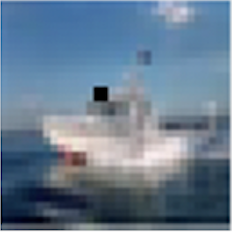
\includegraphics[width=0.99\linewidth]{plotsAistats/CIFAR10_class_boat.png}
  \caption{Masking}
  \label{fig:CIFAR10_boat}
\end{subfigure}
\begin{subfigure}[b]{0.2\textwidth}
  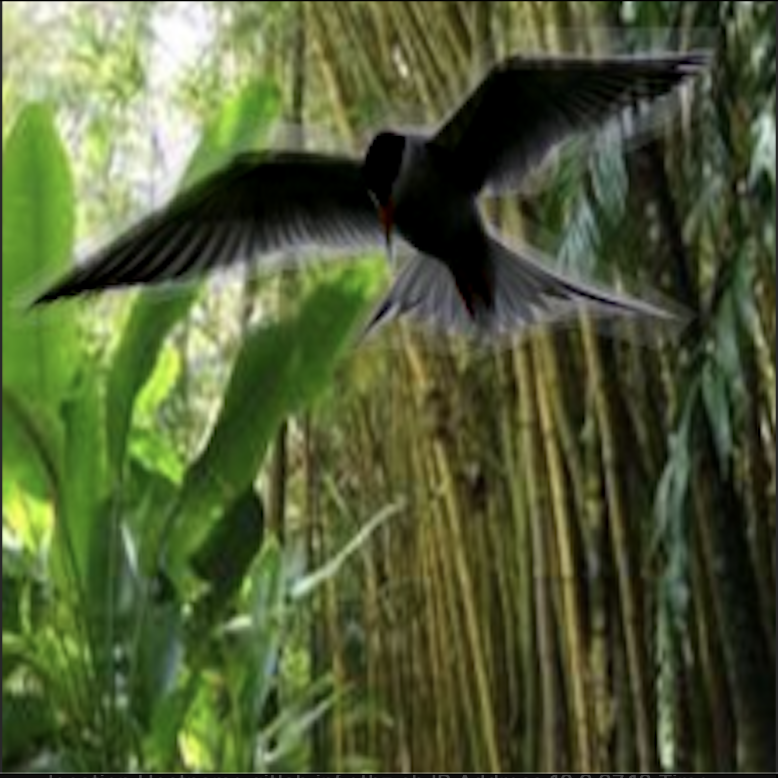
\includegraphics[width=0.99\linewidth]{plotsAistats/light_darker.png}
  \caption{Illumination}
  \label{fig:WB_light_dark}
\end{subfigure}
\begin{subfigure}[b]{0.2\textwidth}
  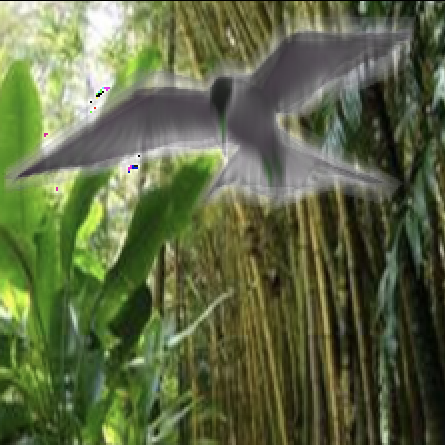
\includegraphics[width=0.99\linewidth]{plotsAistats/water-bird_motion_blurred.png}
  \caption{Motion blur}
  \label{fig:WB_motion_blur}
\end{subfigure}
\begin{subfigure}[b]{0.2\textwidth}
  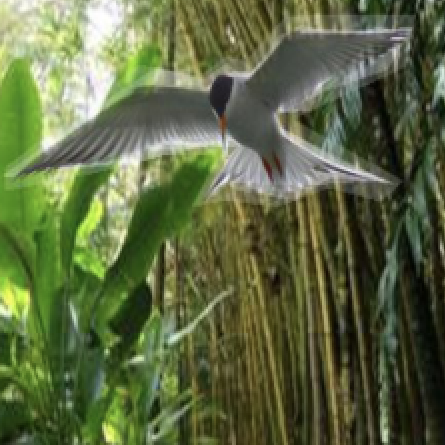
\includegraphics[width=0.99\linewidth]{plotsAistats/waterbird_original_example.png}
  \caption{Original}
  \label{fig:fig:WB_original}
\end{subfigure}
\caption{Examples of \nameofattacks on CIFAR10 and the
  Waterbirds dataset. In Figure \ref{fig:CIFAR10_boat}, we corrupt the image with a black mask of size $2 \times 2$ and in Figure \ref{fig:WB_light_dark} and \ref{fig:WB_motion_blur} we change the lighting conditions (darkening) and apply motion blur on the bird in the image respectively. 
  %with a kernel of size $\motionblurkernel= 15$. 
  All perturbations effectively reduce the information about the class in the images: they are the result of \nameofattacks.}
\label{fig:sig_att_examples}
\end{center}
\vskip -0.2in
\end{figure}


In this paper, we question the efficacy of adversarial training to increase
robust accuracy for \nameofattacks.
In particular, we show that adversarial training not only increases standard test error as noted in \cite{zhang19, tsipras19, Stutz19, raghunathan20}), but surprisingly,
%% Even though adversarial training is widely known to decrease standard accuracy (see e.g. \cite{zhang19, tsipras19, Stutz19, raghunathan20}), none of these works question its benefits on robust generalization.
%% This phenomenon is related to the trade-off between standard and robust accuracy as
%% studied in \cite{zhang19, tsipras19, su18, madry18, raghunathan20,
%%   yang20, Stutz19}, which show that standard accuracy suffers from
%% adversarial training. While in these works robust accuracy is simply assumed
%% to still benefit from AT,
%In this paper we show that this is in fact a misbelief:
\begin{center}
 \emph{adversarial training may even increase the robust test error compared to standard training!}
\end{center}
%% Figure~\ref{fig:teaserplot} depicts the robust accuracy of classifiers
%% obtained by standard and adversarial training on subsampled CIFAR10
%% datasets attacked by $2\times 2$ black masks.  We observe that
%% choosing $\epstrain = \epstest$ is not optimal for robust test
%% accuracy.
Figure \ref{fig:teaserplot} illustrates the main message of our paper for CIFAR10 subsets: Although adversarial training
outperforms standard training when enough training samples are available, it is inferior %increases the robust  than standard training
in the low-sample regime.  
%as shown in Figure~\ref{fig:eps_logreg} and Figure~\ref{fig:waterbirds_light_d_n}, 
%% This observations is consistent across different datasets, models and
%% different types of perceptible perturbations. 
%% , the \emph{larger} $\epstrain$, the higher the robust
%% error.
More specifically, our contributions are as follows:
\begin{itemize}
\item We prove that, almost surely, adversarially training a linear classifier on separable data yields a monotonically increasing robust error as the perturbation budget grows. 
%we increase the adversarial training budget 
%\fy{starting from zero vs. compared to standard training} (standard training), the robust error of linear classifiers monotonically increases for separable data.
%We prove for maximum-margin linear classifiers that \jc{compared to standard training,} almost surely, the robust \jc{and standard} error monotonically increase with increasing adversarial training budget. 
We further establish high-probability non-asymptotic lower bounds on the robust error gap between adversarial and standard training.
  % that increase with $d/n$ until a reasonable threshold; the regime where the standard classifier achieves reasonable standard accuracy. 
\item Our proof provides intuition for why this phenomenon is particularly prominent for \nameofattacks in the small sample size regime. %Notably, the explanation also holds for noiseless settings. \fy{without label noise}
%\fy{somehow I don't know where to move this next sentence, doesn't fit anywhere} Notably, it would \jc{provide one explanation for why} adversarial training can hurt robust generalization even when the observed data is noiseless. \jc{As you write it now is quite nice. I like it}
  %% Using intuition from our theoretical results we provide a visual explanation for this phenomenon  that transfers to other datasets.
\item We show that this phenomenon occurs on a variety of real-world datasets and perceptible \nameofattacks in the small sample size regime.
  %the robust error increases with increasing adversarial training strength. 
\end{itemize}

%% We prove that this phenomenon for linear models but
%% show that it also holds for real-world models trained with neural
%% networks across datasets and is particularly pronounced in the
%% high-dimensional regime where $d/n$ is large.
%% Our contributions are as follows:


